\documentclass{article}
\usepackage[utf8]{inputenc}
\usepackage{indentfirst}
\usepackage{biblatex}
%% Language and font encodings
\usepackage{graphicx}
\usepackage[english]{babel}
\usepackage{csquotes}
%%\usepackage[utf8x]{inputenc}
\usepackage[T1]{fontenc}
\usepackage{listings}
\usepackage{color} %red, green, blue, yellow, cyan, magenta, black, white
\definecolor{mygreen}{RGB}{28,172,0} % color values Red, Green, Blue
\definecolor{mylilas}{RGB}{170,55,241} 

%% Useful packages
\usepackage{amsmath}\usepackage{graphicx}
\usepackage[colorlinks=true, allcolors=blue]{hyperref}
\usepackage{enumitem}
\usepackage{mleftright}
\usepackage{setspace}
\usepackage{wrapfig}
\usepackage{geometry}
 \geometry{
 a4paper,
 total={170mm,257mm},
 left=20mm,
 top=20mm,
 }


\usepackage{natbib}
\bibliographystyle{unsrtnat}


\title{\Huge News Article Classification}
\author{Lauren Contard, Archit Datar \\ 
Yue Li, Robert Lumpkin, Haihang Wu}
\date{}

\addbibresource{FinalReport.bib}
\doublespacing

\begin{document}

\begin{singlespace}
    \maketitle
\end{singlespace}


\section{Introduction and Problem Statement}

\section{Methods}

\subsection{ML-kNN}
ML-kNN (Multi-label k nearest neighbors) is derived from the traditional k nearest neighbors (kNN), except for the multi-label case. While the goal of the traditional kNN algorithm is to predict whether class of the test sample based on the classes of its k nearest neighbors, the goal of ML-kNN is to predict multiple classes based on the classes of the k nearest neighbors of the test point. For the unseen data point, its nearest neighbors are identified. Then, based on the number of neighboring instances belonging to each possible class, maximum a posteriori (MAP) principle is utilized to determine the label set for the unseen instance. 

ML-kNN is used in a variety of problems, such as, text categorization \autocite{McCallum99multi-labeltext}, where each document may belong to several topics, such as the use case for our project. Apart from this, it can also be useful in areas such as functional genomics where each gene may be associated with a set of functional classes \autocite{KernelMulti-labelClassification}, and in image classification, where each image could have multiple genres.\autocite{Boutell04learningmulti-label}  

%%Questions: 1. How were $P(H_1) and P(E | H) derived? Wasn't able to understand very well. 2. What would be wrong with simply considering this as Q separate classification problems? What exactly do we mean by "correlations between labels" and how do they manifest themselves mathematically?$ 
%%Comments: Somehow, the order of citations is reversed. Not sure why that is happening. Probably due to some argument of BibLatex? 

\subsection{Linear Dimension Reduction (PCA)}

\subsection{Nonlinear Dimension Reduction (ANN Autoencoder)}

In addition to reductions in dimension due to PCA, we also implement an ANN autoencoder (see section 2.4 for an introduction to ANNs). Autoencoders can learn data projections with suitable dimensionality and sparsity limitations that are more useful than other fundamental methods such as PCA, which only allow for linear data representations \autocite{Alkhayrat}.

\begin{wrapfigure}{r}{0.5\textwidth}
    \begin{center}
        \raisebox{0pt}[\dimexpr\height-1.95\baselineskip\relax]{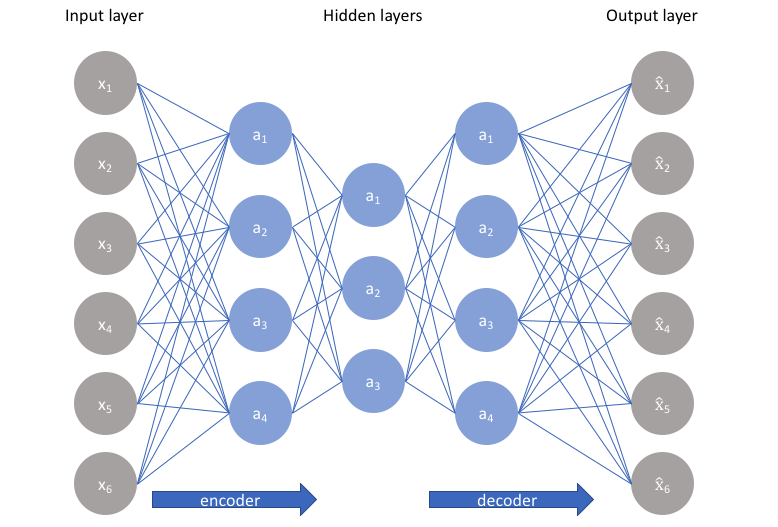
\includegraphics[width=0.5\textwidth]{autoencoder_diagram.png}}
    \end{center}
\end{wrapfigure}

This nonlinear dimension reduction is done by by training a feed forward neural
network to perform the identity mapping, where the network inputs are reproduced
at the output layer. The network contains an internal “bottleneck” layer (containing fewer nodes than input or output layers), which forces the network to develop a compact representation of the input data, and two additional hidden layers \autocite{Kramer}. Look to the diagram to the right, for a visualisation of this set-up. 

The particular network that we trained had three hidden layers, as in the diagram. The first, second and third hidden layers are of dimensions $128$, $64$, and $128$, and use the activations tanh, ReLu, and sigmoid, respectively. Training was performed using Adam optimization, MSE loss, and over $400$ epochs. After training, the generated encodings were used to repeat our model fitting procedures for both the binary-relevance KNN and ML-KNN algorithms. 


\subsection{Artificial Neural Networks (Feed-Forward \& Recurrent)}
Approaches utilizing different artificial neural networks are also utilized in our project. Inspired by biological nervous systems, neural networks date back to the first half of the $20^{th}$ century with works such as those by McCulloch and Pitts, which could model simple logical operations \autocite{Piccinini}. Since most subsequent work in the following two decades centered around single layer networks, the power of neural networks was restricted to linearly separable problems. This excluded the possibility of learning even simple functions like XOR, which required a second layer \autocite{NNLM}. In the early 1980s, research on neural networks resurged largely due to successful learning algorithms for multi-layer neural networks and are used today for various tasks such as computer vision, associative memory, representation learning, NLP, etc..

For our project, we tried implementing both feed forward and recurrent neural network architectures. The feed forward architectures were trained on $2094$ dimensional tf-idf vectors. The recurrent networks were trained on padded sequences of integers corresponding to sequences of the processed tokens from the paragraphs; urls, punctuation, and stop words were all removed. 

Training was performed, using two different loss functions. The standard binary cross entropy loss function was used, in addition, to the more novel BPMLL (back prop for multilabel learning) loss. The BPMLL loss function requires instances to have at least one label. Thus, on the one hand, we trained both cross entropy and BPMLL models on such a reduced dataset in addition to training just cross entropy models on the full dataset. 

The BPMLL loss function aims to leverage correlations between labels by evaluating the error as a function of pairwise errors between labels. Namely, the loss function is given by:

$$
    E = \sum_{i = 1}^m E_i = \sum_{i = 1}^m \frac{1}{|Y_i| |\overline{Y}_i|} \sum_{(k,l) \in Y_i \times \overline{Y}_i} \exp(-(c_k^i - c_l^i))
$$

where $c_j^i = c_j(x_i)$ is the output of the network on $x_i$ on the $j^{th}$ class. The back propagation algorithm is derived in the same manner is for a cross entropy or MSE loss. Details are ommitted here, but can be found in \autocite{bpmll}.

All of our networks utilize the same optimization algorithm (Adam optimization). All of our feed forward networks utilize the same architectures; the first hidden layer is of size 32 with ReLU activation, dropout regularization with drop probability of $0.5$, and an output layer of size $13$ (the number of labels) with sigmoid activations. On the reduced dataset, all of our RNN models utilize the same bidirectional LSTM architecture. On the full dataset, all of our models utilize the same single-directional LSTM architecture.

\subsection{Threshold Function Learning}

\section{Results}

\subsection{ML-KNN Results}

\subsection{Artificial Neural Network Results}

\section{Discussion \& Conclusions}

\newpage
\printbibliography

\end{document}

